\documentclass[output=paper]{langsci/langscibook}
\ChapterDOI{10.5281/zenodo.4680296}
\author{Dalina Kallulli\affiliation{University of Vienna}}
\title{Voice morphology (mis)behaving itself}


\abstract{This paper reconsiders some core issues on the morphosyntax and
    semantics of deponents, and what I contend are their counterparts in
    languages with no fully-fledged voice paradigms, namely pseudo-reflexives
    in \ili{Germanic} and \ili{Romance}. In particular, I show that non-active voice and
    reflexive marking in these constructions functions as a verbalizer,
    specifically on the roots of these verbs, which are nominal. Consequently,
    at least some roots seem to be categorial, and their category and other
    selectional features (such as non-causative semantics) relevant for Merge.
    Thus, the paper provides novel evidence for the view that roots have
    meaning, and in particular, for the existence of entity denoting roots.}

\begin{document}\glsresetall
\maketitle

\section{Introduction}\label{sec:10.1}

While the literature on non-active (versus active) voice morphology in
languages with two distinct conjugational paradigms such as \ili{Latin}, \ili{Albanian} and
Greek has been prolific, in this paper I focus on a particular phenomenon that
has not received a great deal of attention, but that to my mind reveals that,
on top of other functions, non-active voice morphology -- and more generally
special morphology in languages devoid of fully-fledged voice paradigms, such
as reflexive morphology in \ili{Romance} and \ili{Germanic} -- acts as a verbalizer, in
which case it is located in the little \emph{v} head (and not in the higher
Voice head). The crucial evidence I discuss comes from \isi{deponent verbs} in
languages such as \ili{Latin}, \ili{Albanian} and \ili{Greek}, as well as from pseudo-reflexive
verbs of the type ‘to behave (oneself)’ across \ili{Germanic} and \ili{Romance}, which for
all intents and purposes, behave like deponents in the aforementioned
languages, as I will show.

The paper is organized as follows. In~\Cref{sec:10.2}, I introduce deponent
and deponent-like verbs, that is, the basic patterns that motivate the present
inquiry. \Cref{sec:10.3} gives a bird’s eye view of the most common
assumptions on the syntax of voice morphology in the current literature. In
\Cref{sec:10.4}, building on my previous work, I present an alternative
analysis, the most far-reaching consequence of which is that it calls into
question the extreme constructionist position according to which roots never
project (and are thus invariably acategorial).

\section{Deponent and deponent-like verbs}\label{sec:10.2}

While voice syncretisms of the sort found in languages like \ili{Albanian}, \ili{Greek},
and \ili{Latin}, which have two distinct conjugational voice paradigms (namely,
active and non-active, the latter used for verbs in the passive\is{passive}, anticausative
and/or reflexive alternation) are well-known -- see for instance (\ref{ex:10.1}a)
vs.\ (\ref{ex:10.1}b) from \ili{Albanian}~-- \isi{deponent verbs} familiar first and foremost
from traditional grammars of \ili{Latin} have featured much less in modern
theoretical syntax, even though recently there has been increased interest in
them (for a thorough review, see \citealt{Grestenberger2014}).

\ea%1
\label{ex:10.1} \ili{Albanian}
    \ea
	\gll    Po    krihem.\\
            \Prog{}  comb.\Fsg.\Nact{}\\
    \glt    (i) ‘I am combing myself.’\\
            (ii) ‘I am being combed (by someone else).’
    \ex
	\gll    Po    kreh        fëmijën.\\
            \Prog{}  comb.\Fsg.\Act{}  child.the\\
    \glt    ‘I am combing the child.’
    \z
\z

Deponent verbs, which have been traditionally characterized as passive\is{passive} in form
but active in meaning and/or as verbs that do not have an active form, are
illustrated through the verb \emph{hortor} ‘I encourage/incite’ in
(\ref{ex:10.2}b) for \ili{Latin}, which as \citet{Grestenberger2018a} notes, can
only appear with passive\is{passive} morphology (i.e.\ there is no *\emph{hortō}) but is
syntactically active and transitive like \emph{amō} ‘I love’, but which unlike
the passive\is{passive} form of \emph{amō,} namely \emph{amor} ‘I am loved’, never means
*‘I am encouraged’. This amounts to saying that \isi{deponent verbs} do not
passivize.\footnote{\textcite{Grestenberger2014,Grestenberger2018a} notes
however that there is a rather small set of \isi{deponent verbs} that do
passivize. I postpone the discussion of these verbs to \Cref{sec:10.4}.}
The \ili{Albanian} examples in \eqref{ex:10.3} further illustrate the point
that deponents do not have formally (i.e. morphologically) active counterparts
(compare with \eqref{ex:10.1}).

\NumTabs{5}
\ea\label{ex:10.2} \ili{Latin}\\%
        \tab{Present, active} \tab{Present, non-active}
    \ea alternating \tab{\emph{am-\textbf{ō}}} \tab{\emph{am-\textbf{or}}}\\
        \tab{\enquote*{I love}} \tab{\enquote*{I am loved}}
    \ex deponent \tab{---} \tab{\emph{hort-\textbf{or}}}\\
        \tab{} \tab{\enquote*{I encourage/incite}}
    \z
    \ex \ili{Albanian}\label{ex:10.3}\\
    \begin{tabular}[t]{@{}lllll@{}}
       & Non-active & & Active & \\
    a. & dergj-\textbf{em} & a$'$. & \llap{*}\emph{dergj} & \\
       & ‘I linger’ & & & \\
    b. & \emph{përgjigj-\textbf{em}} & b$'$. & \llap{*}\emph{përgjigj} & \\
       & ‘I answer’ & & & \\
    c. & \emph{kreno-h-\textbf{em}} & c$'$. & \llap{*}\emph{kreno-\textbf{j}} & \\
       & ‘I take pride in’ & & & \\
    d. & \emph{lig-\textbf{em}} & d$'$. & \llap{*}\emph{lig} & \\
       & ‘I weaken’ & & & \\
    e. & \emph{pendo-h-\textbf{em}} & e$'$. & \llap{*}\emph{pendo-\textbf{j}} & \\
       & ‘I regret’ & & & \\
       & \dots & & & \\
    \end{tabular}
\z

Furthermore, unlike in \ili{Latin}, \isi{deponent verbs} in \ili{Albanian} are invariably
intransitive, i.e.\ they cannot combine with a direct object bearing accusative
case, though some may combine with dative\is{dative case} objects, as shown in
\eqref{ex:10.4}.\footnote{Not all \isi{deponent verbs} in \ili{Latin} are transitive either,
but crucially, unlike in \ili{Albanian}, some are. See also~\Cref{sec:10.4}.}

\ea%4
    \label{ex:10.4} \ili{Albanian}
    \ea[]{
	\gll  Do  t’u            përgjigjem    pyetjeve.\footnotemark\\
      \Fut{}  \Sbjv.\Cl.\Dat.\Tpl{}  answer questions.\Dat{}\\
      \glt  ‘I’ll answer the questions.’}
      \ex[*]{
	\gll  Do  t’i            përgjigj      pyetjet.\\
      \Fut{}  \Sbjv.\Cl.\Acc.\Tpl{}  answer questions.\Acc{}\footnotemark\\
    \glt  intended: ‘I’ll answer the questions.’}
    \z
\z
\footnotetext{Dative arguments are invariably clitic doubled\is{clitic
doubling} in \ili{Albanian}.}
\footnotetext{Nominative plural and accusative plural are in fact syncretic in
Albanian.}

Deponent verbs in \ili{Albanian} are thus reminiscent of pseudo-reflexive verbs
across \ili{Romance} and \ili{Germanic} languages, in the sense that the reflexive element
here obviously cannot be interpreted as a direct object the way it may be when
occurring with so-called “inherently reflexive” verbs such as ‘to wash’, ‘to
shave’, or ‘to comb’ across all these languages. To see this, consider the
examples in \eqref{ex:10.5} through \eqref{ex:10.10}. Crucially, unlike in
(\ref{ex:10.5}a), (\ref{ex:10.7}a) and (\ref{ex:10.9}a), the reflexive element in
(\ref{ex:10.6}a), (\ref{ex:10.8}a) and (\ref{ex:10.10}a) cannot be said to
correspond to a logical argument of the verb, as is evidenced by comparing the
grammatical (\ref{ex:10.5}b), (\ref{ex:10.7}b) and (\ref{ex:10.9}b), to the
respective (\ref{ex:10.6}b), (\ref{ex:10.8}b) and (\ref{ex:10.10}b), all of which
are ungrammatical. The conclusion that the ungrammaticality of (\ref{ex:10.6}b),
(\ref{ex:10.8}b) and (\ref{ex:10.10}b) is due to a violation of (some version of)
the theta-criterion is therefore imminent.\footnote{Dutch, which is famous for
two morphological classes of reflexives, namely simple \emph{zich} versus
complex \emph{zichzelf}, constitutes an interesting case in this context, since
pseudo- or \enquote{fake} reflexives (i.e.\ reflexive elements that cannot be
said to instantiate an argument of the verb) are simple, just like reflexive
arguments of verbs of bodily grooming such as \emph{comb}, \emph{wash},
\emph{shave} etc.\ (which are inherently reflexive), and unlike reflexive
arguments of non-inherent reflexive verbs such as \emph{hate} or \emph{love},
which are complex. This is interesting because in languages with full-blown
conjugational paradigms like \ili{Albanian}, \ili{Greek} and \ili{Latin}, a non-inherent
reflexive verb bearing non-active morphology can never have a reflexive
interpretation (see e.g.\ \citealt{Embick1997,Embick:2004b} on reflexives in
\ili{Greek}).

\begin{exe}
    \exi{(i)} \ili{Dutch}\\
    \gll    Jan schaamt zich / *zichzelf.\\
            Jan shames \Refl.\Third{} {} \hphantom{*}\Refl.\Third-\textsc{self}\\
    \glt    \enquote*{John is ashamed (of himself).}
    \exi{(ii)} \ili{Dutch}\\
    \gll    Jan haat *zich / zichzelf.\\
            John hates \llap{*}\Refl.\Third{} {} \Refl.\Third{}-\textsc{self}\\
    \glt    \enquote*{John hates himself.}
\end{exe}}

\ea \multicolsep=.25\baselineskip%5
    \label{ex:10.5} \ili{Italian}
    \begin{multicols}{2}
    \ea
	\gll  Martina  si      lava.\\
      Martina  \Refl.\Third{}  washes\\
    \glt  ‘Martina washes herself.’
    \ex
	\gll  Martina  lava    la camicia.\\
    Martina  washes  the shirt\\
    \glt ‘Martina washes the shirt.’
    \z\end{multicols}
\ex\label{ex:10.6} \ili{Italian}
    \ea[]{
	\gll  Martina  si      arrabbia    spesso.\\
        Martina  \Refl.\Third{}  angers    often\\
    \glt  ‘Martina often gets angry.’}
    \ex[*]{
	\gll  Martina  arrabia  spesso  Piero.\\
         Martina    angers  often    Piero\\
    \glt    intended: ‘Martina often angers Piero.’}
    \z
\ex \label{ex:10.7} \ili{German}
    \begin{multicols}{2}
    \ea
	\gll  Martina  wäscht  sich.\\
        Martina  washes  \Refl.\Third{}\\
    \ex
	\gll  Martina  wäscht  das Hemd.\\
        Martina  washes  the shirt\\
    \z\end{multicols}
\z

\ea\label{ex:10.8} \ili{German}
    \ea[]{
	\gll    Ich  schäme  mich.\\
            I    shame  me/myself\\
    \glt    ‘I am ashamed of myself.’}
    \ex[*]{
	\gll    Ich  schäme  dich        /  (die) Martina.\\
            I    shame  you/yourself  {}  \hphantom{(}the Martina\\}
    \z
\z

\ea\label{ex:10.9}
    \ea[]{John washed (himself).}
    \ex[]{John washed the child.}
    \z
\z

\ea\label{ex:10.10}
    \ea[]{John behaved (himself).}
    \ex[*]{John behaved the child.}
    \z
\z

The question then arises what the role of the reflexive element in examples
such as (\ref{ex:10.6}a), (\ref{ex:10.8}a) and (\ref{ex:10.10}a)
is. I have argued in previous work that the reflexive element here is the
counterpart of non-active or passive\is{passive} morphology in the class of verbs known
from traditional grammars of \ili{Latin} as \enquote{deponent} verbs, a view that is
at first blush also corroborated by the fact that reflexive morphology is also
involved in building the so-called “short passives” in \ili{Romance} languages,
examples of which are given in (\ref{ex:10.11}) and (\ref{ex:10.12})
for \ili{Italian} and French, respectively.

\ea\label{ex:10.11} \ili{Italian}\\
    \gll Le  fragole      si    mangiano.\\
        the strawberries  \Refl{}  eat\\
    \glt (i) ‘The strawberries are (being) eaten.’\\
        (ii) ‘Strawberries are edible.’
\ex\label{ex:10.12} \ili{French}\\
    \gll Trois maisons  se    sont  louées (*par des touristes) hier.\\
        three houses \Refl{}  are  rented \hphantom{(*}by some tourists yesterday\\
    \glt ‘Three houses were rented (by some tourist) yesterday.’
\z

I will show that the special morphology of deponent and pseudo-reflexive verbs
is not located in the head of a VoiceP, but in little \emph{v}$^0$, and is thus
as a genuine verbalizer. However, before doing that, in the next section I
quickly review the main lines of analyses of \isi{deponent verbs} in current research
pointing out their merits and their drawbacks, which motivate the alternative
analysis I provide in~\Cref{sec:10.4}.

\section{Analytical state-of-the-art}\label{sec:10.3}

An influential study of \isi{deponent verbs} within modern syntactic thinking is
pro\-vi\-ded in \citet{Embick1997}. Within his overall underspecification
approach (Embick’s study is situated within the framework of \isi{Distributed
Morphology}), the source of the well-known syncretism between (alternating and
non-alternating) unaccusatives,\is{unaccusativity} passives and reflexives, is a particular
syntactic property, namely the lack of an external argument. That is, what
these distinct syntactic constructions have in common is that they all lack an
external argument, and it is precisely this syntactic property that the
syncretic morphology (which \citeauthor{Embick1997} dubs “u-syn\-cre\-tism”) is
sensitive to, or reflects. To deponents, which as discussed, in many languages
share this very same morphology, \citeauthor{Embick1997} assigns a so-called
“class” feature, namely \emph{passive}. More specifically,
\citeauthor{Embick1997} argues that with deponents, unlike in genuine (i.e.\
syntactic) passivization and reflexivization contexts, this feature does not
show up on a functional head\is{functional items}, but rather on a root, where subcatgorization
information and interpretation are not affected.

In spite of the fact that the background of Embick’s approach to the
morphosyntax of voice is a realizational framework, Embick’s approach to
deponents is conceptually eerily similar to lexicalist approaches such as the
one in \citet[121--122]{Kiparsky2005},\footnote{See also
\citet{SadlerSpencer2001}.} who suggests that “passive inflection in \ili{Latin} is a
conjugational feature -- we’ll call it [±Passive] -- which can be lexically
specified, for verb stems as well as for inflectional endings, or left
unspecified”, and who further goes on to state that “[+Passive] inflections
trigger one or more of the operations on the verb’s argument structure [\dots]
forming passives, as well as possibly reflexives, reciprocals, and inchoatives,
depending on further, partly idiosyncratic, properties of the verb”. The
question then also for \citeauthor{Embick1997} is what, if anything, enables
the appearance of this class feature on roots? This question becomes even more
pressing in view of generalizations like those drawn in work by
\textcite{Xuetal2007} on deponents in \ili{Latin}, \citet{Kallulli2013} on deponents
in \ili{Albanian}, and \citet{ZomAle2014} on deponents in \ili{Greek}, according to which
there is no mismatch. Under these approaches, the morphological exponent
faithfully realizes a certain abstract semantic property, i.e.\ \isi{deponent verbs}
in all these languages can form a semantically defined natural class with
other, more obvious instances of non-active morphology after all.  For
instance, in \citet{Kallulli2013} I argue that the fact that
cross-linguistically deponents are overwhelmingly denominal crucially evidences
the canonicity of the non-active form for this class of verbs, since nouns
typically lack external arguments.\footnote{In \citet{Kallulli2013} I also show
    that this is largely the case for pseudo-reflexives in modern \ili{Romance} and
    \ili{Germanic}, too; i.e.  like deponents, pseudo-reflexives are
cross-linguistically overwhelmingly denominal.} I will indeed defend this
proposal here, in particular taking issue with another recent influential
proposal, namely the one in \citet{Grestenberger2014,Grestenberger2018a}, which
I turn to next.\largerpage[-3]

Based on \citet{Grestenberger2014}, \textcite{Grestenberger2018a} provides the
definition of deponency in \eqref{ex:10.13}:

\ea%13
    \label{ex:10.13} Definition of deponency:\\
    In an active/non-active voice system, a deponent is a verb with an agent
    subject that appears in a syntactically active context and is
    morpho\-lo\-gi\-cal\-ly non-active.
\z

Thus, \citeauthor{Grestenberger2014} argues that \isi{deponent verbs}, as a lexical property, project
an agent DP \emph{within} the VP (as opposed to \emph{v}P which in her notation
equals VoiceP). That is, there is an agent, the clause is transitive, but the
context for morphological realization of active exponence (see \eqref{ex:10.14})
is not present, which is what leads \citet{Muller2016b} to classify
Grestenberger’s approach as a “spurious morpho-syntactic” one.\footnote{For
    \citet{Muller2016b}, Grestenberger’s approach belongs to the class of
    spurious morpho-syntactic approaches to deponency because non-active
    morphological realization is tied to the abstract morpho-syntactic property
    of Voice devoid of a DP specifier, and it is this abstract property that
    characterizes regular passive\is{passive} verbs and \isi{deponent verbs} as a natural class.
    Thus, strictly speaking there is no mismatch between form and function,
    even though \citeauthor{Grestenberger2014} herself classifies her approach as involving a
    genuine mismatch given her contention that the agent of deponents is merged
low (i.e. not in Spec of VoiceP, the canonical position where agents are
externally merged).}

\ea%14
    \label{ex:10.14} Post-syntactic rules of morphological exponence:
    \ea Voice triggers non-active morphology if it does not have an agentive DP
        as its specifier
    \ex Voice triggers active morphology if it has an agentive DP as its
        specifier
    \z
\z

More specifically, \citeauthor{Grestenberger2014} argues that the low agent of deponents is the
outcome of a diachronic \isi{reanalysis} process by which a self-benefactive
argument, which is merged below VoiceP as given in \figref{fig:fromex:10.15a}, is
reanalyzed as an agent, as shown in \figref{fig:fromex:10.15b}, where the boxed DP is the
one undergoing the \isi{reanalysis}. The resulting deponent structure is given in
\figref{fig:fromex:10.16}.\footnote{Note that self-benefactive arguments always occur
with non-active morphology in languages like \ili{Latin} and \ili{Greek}. For details, see
\textcite{Grestenberger2014,Grestenberger2018a}.}

\begin{figure}\footnotesize
\begin{subfigure}[b]{.5\textwidth}\centering
    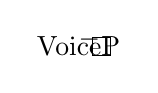
\begin{tikzpicture}[baseline=(root.base)]
        \Tree 	[.\node(root){VoiceP};
                    {Voice\\{}[$-$ext.arg]}
                    [.ApplP\textsubscript{\Ben}
                        \node (ben) [draw] {\Ben};
                        [.Appl\textsubscript{\Ben}
                            Appl\textsubscript{\Ben}
                            [.\emph{v}P
                                \emph{v}
                                [.Root
                                    Root
                                    \textsc{theme}
                                ]
                            ]
                        ]
                    ]
                ]
    \end{tikzpicture}
    \caption{Self-benefactive structure pre-raising\label{fig:fromex:10.15a}}
    \end{subfigure}\begin{subfigure}[b]{.5\textwidth}\centering
    
\begin{tikzpicture}[baseline=(root.base)]
        \Tree 	[.\node(root){VoiceP};
                    {Voice\\{}[$-$ext.arg]}
                    [.XP
                        \node (ag) [draw] {\textsc{agent}};
                        [.X
                            X
                            [.\emph{v}P
                                \emph{v}
                                [.Root
                                    Root
                                    \textsc{theme}
                                ]
                            ]
                        ]
                    ]
                ]
    \end{tikzpicture}
    \caption{Reanalysed deponent pre-raising\label{fig:fromex:10.15b}}
    \end{subfigure}
    \caption{The structure of self-benefactives pre- and post-reanalysis}
\end{figure}

\begin{figure}\footnotesize
\caption{\label{fig:fromex:10.16}Deponent}
    \begin{tikzpicture}[baseline]
        \Tree 	[.TP
                    \node (ag) {\textsc{agent}$_i$};
                    [.VoiceP
                        {Voice\\{}[$-$ext.arg]}
                        [.XP
                            \node (t) {\tuple{\textsc{agent}}$_i$};
                            [.X
                                X
                                [.\emph{v}P
                                    \emph{v}P
                                    [.Root
                                        Root
                                        \textsc{theme}
                                    ]
                                ]
                            ]
                        ]
                    ]
                ]

        \draw [arrow, ->, bend left=60] (t.south) to (ag.south);
    \end{tikzpicture}
\end{figure}

The \ili{Albanian} data in \eqref{ex:10.17} seem to lend support to Grestenberger’s
approach. Specifically, in (\ref{ex:10.17}a), with the non-active verb
\emph{lutem} ‘I beg’, Eva (who bears nominative\is{nominative case} case) is the beggar and Ben
(who bears dative\is{dative case}) the one being begged. In (\ref{ex:10.17}b), with the active
verb \emph{lus} ‘I beg’, again (nominative) Eva is the beggar and Ben, which
crucially bears accusative here, is the one being begged. While the two
sentences feel synonymous, there is a sense in which Eva in (\ref{ex:10.17}a) --
note the existence of non-active morphology here -- feels more
\enquote{affected} than in (\ref{ex:10.7}b), i.e. like pleading with Ben,
thus reflecting a sense of self-beneficial implication. Under Grestenberger’s
approach, this \enquote{affectedness} effect could be said to have been lost
over time (at least with certain verbs), resulting in the same unmarked agent
reading as in (\ref{ex:10.17}b), but with the non-active morphology as a
sort of diachronic remnant.\footnote{Incidentally, Laura
    \citeauthor{Grestenberger2014} (personal communication) confirms that ‘beg’
    and ‘ask’ are definitely verbs that show up as deponents in Ancient \ili{Greek}
    and Sanskrit (mostly with accusative objects).}

\ea\label{ex:10.17} \ili{Albanian}
    \ea
	\gll    Eva i\textbf{u} lut Benit (për muaj me rradhë).\\
            Eva.\Nom{}  \Cl.\Tsg.\Dat.\textbf{\Nact} begged Ben.\Dat{} \hphantom{(}for months on end\\
    \glt    `Eva begged Ben (for months on end).'
    \ex
	\gll    Eva e luti Benin (për muaj me rradhë).\\
            Eva.\Nom{}  \Cl.\Tsg.\Acc{}  begged.\Act.\Tsg{} Ben.\Acc{} \hphantom{(}for months on end\\
    \glt    `Eva begged Ben (for months on end).'
    \z
\z

A potentially problematic aspect of Grestenberger’s approach for data such as
these however lies in her statement that “the non-active morphology of
deponents cannot be motivated in terms of the \emph{synchronic} canonical
functions of non-active morphology. That is, synchronically they do not fall
into any of the categories listed […] (reflexive, self-benefactive,
anticausative, etc)”. At least in \ili{Albanian}, deponents, which in this language
are incompatible with objects bearing accusative case, actually do seem to fall
into some such category associated with the synchronic canonical functions of
non-active morphology (namely: self-benefactive). In other words, the pattern
observed in (\ref{ex:10.17}a) vs.\ (\ref{ex:10.17}b) seems to be productive, as
also replicated in (\ref{ex:10.18}a) vs.\ (\ref{ex:10.18}b).\newpage

\ea\label{ex:10.18} \ili{Albanian}
    \ea
    \gll    Mendohem *(për) {të ardhmen}.\\
            ponder.\Fsg.\Prs.\Nact{} \hphantom{*(}for    future.the.\Acc{}\\
    \glt    ‘I ponder/think about the future.’
    \ex
    \gll    Mendoj (për) {të ardhmen}.\\
            think.\Fsg.\Prs.\Act{}  \hphantom{(}about future.the.\Acc{}\\
    \glt    ‘I think about the future.’
    \z
\z

A solution to this tension might be that the synchronic analysis of data such
as (\ref{ex:10.17}a) and (\ref{ex:10.18}a) might be different from the
languages Grestenberger scrutinizes, especially in view of the
\enquote{affectedness} ingredient in these examples as opposed to
(\ref{ex:10.17}b) and (\ref{ex:10.18}b), respectively. Coupled with the
productivity of the pattern (i.e.\ the alternation) illustrated here and the
fact that deponents in \ili{Albanian} are incompatible with accusative objects, it
seems reasonable to assume that \citet{Grestenberger2018a} wouldn’t have to
analyze cases like (\ref{ex:10.17}a) and (\ref{ex:10.18}a) as deponents
at all, because they are not agentive; recall her definition of deponency in
\eqref{ex:10.13}.\footnote{I am grateful to Laura Grestenberger for
discussing these data and the issues they present with me.} It is precisely in
terms of (lack of) agency that my approach to deponents differs from
Grestenberger’s (as well as from Embick’s). Specifically, I maintain that
Grestenberger’s definition of deponency is not only too narrow in that not all
deponents can be conceived of as agentive predications, but that deponents are
truly non-agentive predications. I discuss this issue in detail among others in
the next section.

\section{Deponents and pseudo-reflexives are unaccusatives}\label{sec:10.4}

Building on my previous work in \citet{Kallulli2013}, I maintain that deponents
and their pseudo-reflexive counterparts in languages with no full-fledged voice
par\-a\-digms are truly unaccusative\is{unaccusativity} predications -- i.e.\ they lack an external
argument. The main evidence for this contention involves the following issues.
Firstly, though \enquote{transitive} deponents (i.e.\ deponents that combine
with objects bearing accusative case) exist both in \ili{Latin}, \ili{Greek} and other
languages with voice paradigms (for details, see
\citealt{Grestenberger2014,Grestenberger2018a}), which is the main if not sole argument motivating the view that
syntactically they are not unaccusative\is{unaccusativity}, not all languages that have deponent
verbs have transitive deponents. Thus, in \ili{Albanian} there are no transitive
deponents, as already mentioned. Secondly, as \citet[590]{Flobert1975} notes,
most of the oldest deponents in \ili{Latin} are intransitive, a fact that is itself
in need of explanation, and that might be construed to reveal the true
(unaccusative) nature of this class of verbs.\footnote{On the emergence and
    development of \enquote{active} deponents in \ili{Latin} see also
    \citet{Cennamo2008}, who notes among other things that full activization of
deponents in this language is attested from the 7th century onwards.}
Similarly, the fact that intransitive deponents in Modern \ili{Greek} far outnumber
transitive deponents, and the fact that the majority of transitive deponents
are verbs that thematically assign experiencer roles \citep{Zombolou2012}, also
speaks for their unaccusative\is{unaccusativity} nature.\footnote{\citet{Zombolou2012} reports
    that 70\% of all \isi{deponent verbs} in this language are intransitive and only
18\% out of 100\% combine with an object bearing accusative case.} Thirdly, the
fact that deponents just like their fake reflexive counterparts in modern
Romance and \ili{Germanic} are largely denominal (see \citealt{Kallulli2013} and
references therein) also speaks for their unaccusative\is{unaccusativity} nature, given that nouns
lack external arguments. Finally, though deponents cannot always combine with
prepositional phrases indicating the presence of an agent or external cause of
an event, some verbs that are clearly derived from such deponents with no
causative semantics (compare (\ref{ex:10.19}a) to (\ref{ex:10.20}a)
below) can however transitivize, as shown in (\ref{ex:10.20}b) which
contrasts with (\ref{ex:10.20}c).\footnote{The prefix \emph{zh-} in
    \ili{Albanian} is a productive antonymizing one analogous to \emph{dis-} in
    \ili{English} and seemingly attaches to various categories, including verbs,
adjectives and nouns.}

\ea\label{ex:10.19} \ili{Albanian}
    \ea
	\gll    Dielli u duk (*nga  Zoti / qielli).\\
    sun \Nact{} appeared \hphantom{(*}from/by God {} sky\\
    \glt    ‘The Sun appeared (*by/from God / the sky).’
    \ex
	\gll    Krenohem (*nga djali) / për / me djalin.\\
            am.proud.\Prs.\Nact{} \hphantom{(*}from/by son.the.\Nom{} {} for {} with son.the.\Acc\\
    \glt    ‘I am proud of my son.’
    \z
\ex \label{ex:10.20} \ili{Albanian}
    \ea[]{
	\gll    Në rregull,  po    \textbf{zh}dukem      atëhere.\\
            in order    \Prog{}  \textbf{dis}appear.\Nact{}  then\\
    \glt    ‘OK, I (will) disappear then.’}
    \ex[]{
	\gll    I \textbf{zh}duka    gjurmët.\\
            \Cl.\Tpl.\Acc{}  disappear  traces\\
    \glt    ‘I made the traces / evidence disappear.’ (i.e. ‘I destroyed the evidence’.)}
    \ex[*]{
	\gll    Duk      diellin / gjurmët.\\
            appear.\Act{}  sun.the {} traces.the\\
    \glt    ‘I make the sun/the traces (i.e. evidence) appear.’}
    \z
\z

The very same transitivization process as in (\ref{ex:10.20}b) is also
attested with pseudo-reflexives in \ili{Romance} and \ili{Germanic}, as illustrated in
\eqref{ex:10.21} for \ili{Italian} and \eqref{ex:10.22} for
German.\footnote{As an anonymous reviewer correctly points out, the \ili{German}
prefix \emph{be}- is a transitivizing one and also attaches to non-deponent
forms of course, which is however irrelevant in the context of the present
discussion.}

\ea\label{ex:10.21} \ili{Italian}
    \ea[]{
	\gll    quando Dio  *(si) vergogna  degli uomini e gli uomini  *(si) vergognano di Dio\\
            when    God \hphantom{*(}\Refl{} shamed of-the men and the men \hphantom{*(}\Refl{} shamed of God\\
    \glt    ‘when God is ashamed of men and men are ashamed of God’}
    \ex[*]{
	\gll    Gli uomini hanno vergognato il Dio\\
            the men have shamed the God\\
    \glt    ‘Men have put God to shame’}
    \ex[]{
	\gll    Gli uomini hanno \textbf{s}vergognato il Dio\\
            the men have shamed God\\
    \glt    ‘Men have put God to shame’}
    \z
\ex \label{ex:10.22} \ili{German}
    \ea[]{
	\gll    Ich  schäme  mich.\\
            I    shame  me/myself\\
    \glt    ‘I am ashamed of myself.’}
    \ex[*]{
	\gll    Ich  schäme  dich.\\
            I    shame  you/yourself\\
    \glt    ‘I put shame on you.’ / ‘I put you to shame.’}
    \ex[]{
	\gll    Ich  \textbf{be}schäme  dich.\\
            I    ashame    you/yourself\\
    \glt    ‘I put shame on you.’ / ‘I put you to shame.’}
    \z
\z

Taken together, these facts suggest that the function of non-active morphology
in deponents and, accordingly, of reflexive morphology in languages that do not
have full-fledged voice paradigms, is that of a verbalizer, i.e. verbalizing
nominal roots, an idea which is also theoretically appealing, since what we
know about nouns is that just like unaccusative\is{unaccusativity} (and passive) verbs, they lack
external arguments, thus making the appearance of non-active/reflexive
morphology be the canonical and therefore expected rather than the
non-canonical, unexpected form.

One question that arises, however, concerns the so-called “transitive”
\citep{Embick1997} deponents of the \emph{sequor} ‘I follow’ type, which as
mentioned can combine with an accusative object (and which
\citeauthor{Grestenberger2014} argues to be truly
“agentive”).\footnote{Incidentally, as an anonymous reviewer reminds me,
evidence for an unaccusative\is{unaccusativity} approach to ‘follow’-type verbs is clearer in
German, where it takes a dative\is{dative case}, not an accusative, object.} Following a
suggestion originally due to \citet{Embick1997}, which he however eventually
discards, but which has more recently been picked up in \citet{Alexiadou2013},
\citet{Kallulli2013} and \citet{ZomAle2014}, I uphold that transitive
non-alternating non-active verbs can be analyzed synchronically as verbs taking
experiencer arguments (note that according to \citet{Pesetsky1995} experiencer
arguments are arguments of the root), specifically as dyadic unaccusative
(stative) psych predicates.\footnote{See also \citet{Zombolou2012}, who points
    out that the subject of the majority of transitive deponents in Modern
    \ili{Greek} (transitive deponents combining with an accusative object make up
18\% of deponents in this language) are experiencers.} As mentioned earlier,
this line of reasoning has however been newly rejected in
\textcite{Grestenberger2014,Grestenberger2018a}, who contends that there is
indeed a small class of truly agentive deponents. Grestenberger’s main
arguments are the following. First, reiterating Embick’s observations which
eventually led him to discard the idea that transitive deponents are psych
verbs, she points out that with some psych-verbs, both an agentive and a
psychological reading is possible in Modern \ili{Greek}. Under what she refers to as
“the agentive reading”, as in (\ref{ex:10.23}a) which contains an
animate\is{animacy}
subject, the object does not have to be clitic doubled, while under the
psychological reading in (\ref{ex:10.23}b) (note that the subject is
inanimate), the object needs to be clitic doubled.\is{clitic doubling}

\ea\label{ex:10.23} \ili{Greek}
    \ea
	\gll    I    Maria    enohli  ton  Petro.\\
            the  Maria.\Nom{}  bothers  the Petro.\Acc{}\\
    \glt    ‘Maria bothers Petro.’
    \ex
	\gll    Ta    epipla    *?(ton)    enohlun  ton  Petro.\\
            the  furniture.\Nom{} \hphantom{*?(}him.\Cl.\Acc{}  bothers the.\Acc{}  Petro\\
    \glt    ‘The furniture bothers Petro.’
    \z
\z

Transitive agentive deponents like \emph{hriazome} ‘need’ pattern with the
so-called “agentive” reading and do not require \isi{clitic doubling}, as shown in
\eqref{ex:10.24}. \citeauthor{Grestenberger2014} takes this to indicate that the subject of
\emph{hriazome} is therefore an agent rather than a cause/theme.

\ea\label{ex:10.24} \ili{Greek}\\
    \gll    I    Maria    hriazete  ton  Petro.\\
            the  Maria.\Nom{}  needs the.\Acc{}  Petro\\
    \glt    ‘Maria needs Petros.’
\z

While these judgments seem clearer for some \ili{Greek} speakers than for others, all
they show is that the distinction between animate and inanimate\is{animacy} subjects has
some bearing on \isi{clitic doubling} of the object.\footnote{I thank Artemis
Alexiadou (personal communication) for discussing these data with me.} Jumping
from such data to the conclusion that the relevant contrast (highlighted in
(\ref{ex:10.23}a) vs. (\ref{ex:10.23}b)) is due to the agentivity of
the subject in (\ref{ex:10.23}a), is unwarranted, since Maria could equally
well be an actor unintentionally causing bother to Petro, i.e. Maria could be
an actor but not an agent. Likewise, in \eqref{ex:10.24} Maria might indeed
need Petro without intending or even wanting to. In other words, what these
examples show, is just that \isi{clitic doubling} of the object is affected by the
(in)animacy of the subject but they can certainly not be used as a test for
agentivity, since participants capable of willful agency might always act
unintentionally.\footnote{For details on (animate) actors versus (intentional)
agents and their representation, see \citet{Demirdache1997} and
\textcite{Kallulli2006b,Kallulli2007}.}  Similarly, Embick’s observation
reiterated by \citeauthor{Grestenberger2014} that transitive deponents pattern as non-psych
verbs in triggering clitic left-dislocation\is{clitic left dislocation} is not
any more conclusive of the agentivity of transitive deponents.

Secondly, as I point out in \citet{Kallulli2007} in a different context,
Grestenberger’s claim that so-called “agent-oriented” adverbs expressing
intention or volition only modify agentive predicates is cross-linguistically
contradicted by data like those in \eqref{ex:10.25} for \ili{Italian} and
\eqref{ex:10.26} for \ili{German}, which specifically demonstrate that
unaccusative\is{unaccusativity}
syntax is not incompatible with such adverbs:

\ea\label{ex:10.25} \ili{Italian} \parencite{FolliHarley2006}
    \ea
	\gll    Gianni é  caduto  /  *ha  caduto  apposta.\\
            Gianni is fallen {} \hphantom{*}has  fallen    on.purpose\\
    \ex
	\gll    Gianni é rotolato  /  *ha  rotolato  giu  apposta.\\
            Gianni is rolled {} \hphantom{*}has  rolled    down  on.purpose\\
    \z
\ex\label{ex:10.26} \ili{German}\\
    \gll    Peter ist / *hat  absichtlich  eingeschlafen.\\
            Peter is {} \hphantom{*}has  deliberately fallen.asleep\\
    \glt    ‘Peter fell asleep on purpose.’
\z

Grestenberger’s strongest argument for the agentive status of (transitive)
deponents comes from languages like Vedic and in some cases Ancient \ili{Greek},\linebreak
which have a trivalent voice system, where one can distinguish among other
things between deponents and passives on the basis of morphology. In other
words, Grestenberger’s strongest argument is that there are languages in which
deponents may passivize. While the data she provides from Vedic (and Ancient
Greek) seem to indicate this, these data have the potential to bring down
Grestenberger’s own system, since one would have to assume a Passive head on
top of the voice head, which makes these languages similar to \ili{English}, \ili{German}
or \ili{Hebrew} (see \citealt{Alexiadou2013} and \citealt{AlexiadouEtAl2015}), but
which in turn contradict her own observation that there are no deponents in
\ili{English}/\ili{German}. In even more recent work, \citet{Grestenberger2018b} argues
however that these languages do not have a higher Passive head, and that what
looks like a passive\is{passive} suffix is between the root and the Voice head, in the
position where we usually find \emph{v}, which has recently been analyzed as
verbalizing morphology (see \citealt{AlexiadouEtAl2015} and references
therein). In other words, the passive\is{passive} head in such trivalent systems selects
roots rather than \emph{v} or Voice, and seems to suppress the projection of
higher arguments (that is, agents). While \citeauthor{Grestenberger2014}
maintains that this holds as a diagnostic of agentivity in deponents because
this passive\is{passive} suffix blocks the projection of both non-deponent and deponent
agentive verbs alike, it should be noted that she thus directly provides
independent evidence for my central claim in this paper, namely the existence
of verbalizing voice morphology close to the root, which moreover seems rather
similar in function to non-active and/or reflexive morphology in deponents (and
elsewhere) in that it blocks the projection of higher
arguments.\footnote{Grestenberger provides one more argument from agent nouns
    for her claim that deponents are agentive predicates. Since the discussion
    of this issue is rather complex, and the evidence is confounding and
therefore non-conclusive, I will for reasons of space not dwell on it here.}
Notice also that my claim that non-active and/or reflexive morphology can on
top of other things also function as a verbalizer (specifically in the case of
deponents and/or fake reflexives), fills in a gap in the voice typology
provided in \citet{Schäfer2008}, which is summarized in \eqref{ex:10.27}.
According to this picture, (\ref{ex:10.27}a) generates so-called
“\textsc{se}-reflexives” such as (the \ili{Romance} and \ili{Germanic} counterparts of)
\emph{wash} \emph{oneself}, which are semantically and syntactically transitive
predicates.\footnote{Note that this does not include fake reflexives.} In
contrast, the semantically intransitive but syntactically transitive structure
in (\ref{ex:10.27}b) generates \textsc{se} (i.e.\ reflexively) marked
anticausatives as in \ili{Romance} (e.g.\ \emph{se casse} ‘breaks’ in \emph{Le vase
\textbf{se} casse} ‘The vase breaks’) or \ili{Germanic} (e.g.\ \emph{Die Tür öffnet
\textbf{sich}} ‘The door opens’), with the reflexive marker being an expletive\is{expletives}
argument. The statements in (\ref{ex:10.27}c) and (\ref{ex:10.27}d) are
self-explanatory: (\ref{ex:10.27}c) refers to the general passive\is{passive} voice,
introduces an external argument θ-role but lacks a D-feature, and the external
argument must remain implicit but can be taken up via \emph{by}{}-phrase,
whereas (\ref{ex:10.27}d) refers to the Voice head for marked
anticausatives in languages like \ili{Greek} (i.e.\ anticausatives bearing non-active
rather than active morphology), with the expletive\is{expletives} not introducing a
θ-role.\footnote{Note that (\ref{ex:10.27}d) differs from the active
expletive Voice in (\ref{ex:10.27}b), as it does not project a specifier.}

\ea\label{ex:10.27}
    \ea   {}[\textsubscript{TP} \emph{T} [\textsubscript{VoiceP} DP\textsubscript{\textsc{agent}} \emph{Voice} [\textsubscript{\emph{v}P} \emph{v} SE\textsubscript{\textsc{patient}} ]]]
    \ex   {}[\textsubscript{TP} \emph{T} [\textsubscript{VoiceP} SE\textsubscript{\textsc{expl}} \emph{Voice} [\textsubscript{\emph{v}P} \emph{v} DP\textsubscript{\textsc{theme}} ]]]
    \ex   Thematic passive\is{passive} Voice
    \ex   Non-thematic (expletive) passive\is{passive} Voice
    \z
\z

It should thus be obvious from the preceding discussion that what the voice
typology in \eqref{ex:10.27} does not cover is one of the core patterns
discussed in the present paper, namely pseudo-reflexives across \ili{Romance} and
Germanic.

It is important to note that the fact that deponents are largely denominal does
not entail that if a verb is denominal, it is deponent (i.e.\ there is an
implication, but there is no equivalence). Indeed denominals have correctly
been claimed to be the historical source for unergatives\is{unergativity} in languages like
English and potentially universally. Interestingly however, unlike (denominal)
unergatives,\is{unergativity} denominal deponents in \ili{Albanian} do not involve nominal morphology.
That is, the noun in the latter class of verbs is just the historical source.
Crucially, as \textcite[139]{Xuetal2007} point out for \ili{Latin} deponents but the
point is more general (see \citealt{Kallulli2013}), \ili{Latin} denominal or
deadjectival verbs differ in form depending on whether they have a causative
sense: “[t]hose with causative senses tend to be active, while those that fall
into general non-causative semantic categories such as ‘to act or to be x’, ‘to
act like y’, ‘to give or make (with a sense of creation) z’, ‘to use z’, and
‘to get z’ tend to assume deponent forms”. This is precisely why non-active
rather than active morphology is used as a default verbalizer in these
(non-causative) contexts, but this does not mean that active morphology cannot
be used as a verbalizer in other contexts, such as causative ones, where indeed
it is the default one. This notion of \enquote{defaultness} is closely
tied to \citegen{Kallulli2007} system summarized in~\Cref{tb:10.1}, with
the primitive features in this system being privative.

\begin{table}[htpb]
    \centering
    \begin{tabular}{lll}
    \lsptoprule
    & Features in \emph{v}$^0$  & \\
    \midrule
    a.  & [$+$activity]             & \emph{Ben ate the apple.}\\
    b.  & [$+$activity]             & \emph{The apple was eaten by Ben.}\\
        & [$-$external argument]    & \\
    c.  & [$+$cause]                & \emph{The pressure cracked the window.}\\
    d.  & [$+$cause]                & \emph{The window cracked (from the pressure).} \\
        & [$-$external argument]    & \\
    e.  & [$+$cause]                & \emph{John cleaned the table.}\\
        & [$+$activity]             & \\
    f.  & [$+$cause]                & \emph{The table was cleaned (by John).}\\
        & [$+$activity]             & \\
        & [$-$external argument]    & \\
    g.  & [$-$external argument]    & \emph{John arrived.}\\
    \lspbottomrule
    \end{tabular}
    \caption{Feature system in \textcite{Kallulli2007}}\label{tb:10.1}
\end{table}

Indeed, the very existence of the grammatical sentences (\ref{ex:10.20}b),
(\ref{ex:10.21}c) and (\ref{ex:10.22}c) above as opposed to the
ungrammaticality of (\ref{ex:10.20}c), (\ref{ex:10.21}b) and
(\ref{ex:10.22}b) across \ili{Albanian}, \ili{Italian} and \ili{German}, respectively, is
evidence for the correctness of my core contention here.

\section{Conclusion}\label{sec:10.5}

In this paper, I have reconsidered some core issues on the morpho-syntax and
semantics of deponents and what I have contended are their counterparts in
languages with no fully-fledged voice paradigms, namely pseudo-reflexives. In
particular, I have shown that non-active voice and reflexive marking can
sometimes function as a verbalizer, specifically on \enquote{deponent} roots,
which are nominal. Thus, a far reaching conclusion is that at least some roots
seem to be categorial, and their category and other selectional features (such
as non-causative semantics) relevant for \isi{Merge}. At the very least we have
seen novel evidence for the view that roots have meaning and that specifically
there are entity denoting roots, as argued in \citet{Harley2005,Levinson2007}
and others.

\makeatletter
{\renewenvironment{theglossary}%
  {\begin{multicols}{3}\raggedright\def\@gls@prevlevel{-1}}{\par\end{multicols}}
  \printchapterglossary{}}
\makeatother

\section*{Acknowledgements}

During Eric Reuland’s talk at the Budapest conference on Minimalist approaches
to syntactic locality in August 2009, turning to Ian sitting next to me I ask
tongue in cheek whether he knows anything about the etymology of the verb
\textit{behave}, noting that it contains both \textit{be} and \textit{have}.
Ian laughs, ponders for an instant, and says: “You might be right, it sounds \ili{Germanic},
but the moment you think of \textit{behaviour} you have Romance”. Indeed one does, as
pseudo-reflexives in \ili{English} seem to be latinate:
absent\slash behave\slash perjure\slash vaunt\slash\dots{} oneself.
(Here’s to many\linebreak more Tokajis, dear Ian!)

{\sloppy\printbibliography[heading=subbibliography,notkeyword=this]}
\end{document}
